\documentclass[a4paper]{article}
%\documentclass[a4paper,10pt]{scrartcl}

\usepackage[utf8]{inputenc}
\usepackage{graphicx}

\title{Linklets}
\author{}
\date{}

\pdfinfo{%
  /Title    ()
  /Author   ()
  /Creator  ()
  /Producer ()
  /Subject  ()
  /Keywords ()
}

\begin{document}
\maketitle

\paragraph{} Linklets are the new units of compilation in Racket, that
constitute the core language that is consumed by the compiler. Given a
Racket module, the macro expander (that implements among others the
Racket macro system and the module system) outputs numerous code
bundles in the form of linklets, each corresponding to a chunk of code
that lives in different phases (e.g. expansion, run-time etc.). The
compiler, then, consumes these linklets and proceeds with the
pipeline. The separation of expansion and compilation makes it easy
for Racket to have different compilers and run-times. Any
compiler/run-time that has a small layer that implements the linklet
functionality (e.g. compile, instantiate linlets) can consume these
linklets and become a Racket implementation, e.g. Chez Scheme.
\cite{racketcs-icfp-2019}

\paragraph{} This document explains the linklet forms, how they
operate and how they are used to turn Pycket from being a Racket
compiler into a full implementation.

\section{Linklet Form}

\begin{figure}[h!]
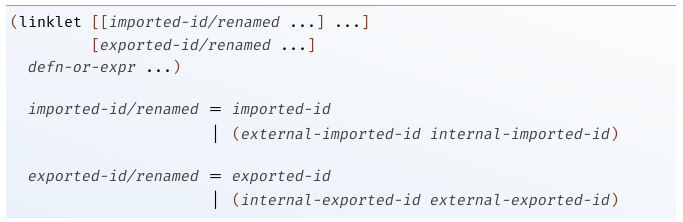
\includegraphics[scale=0.5]{img/linklet-grammar.png}
\caption{Linklet Grammar}
\label{fig:linklet-grammar}
\end{figure}


\begin{figure}[h!]
\begin{center}
\includegraphics[scale=0.6]{linklet-source}
\caption{Linklet Source}
\end{center}
\end{figure}

\paragraph{} Linklets are basic $\lambda$-like forms that consume
(i.e. import) and produce (i.e. export) variables instead of
values. As shown in Figure \ref{fig:linklet-grammar}, linklets may
rename imports as well as exports. The \emph{defn-or-expr} is an
expression of ``fully expanded programs'' (FIXME).

\section{Instantiating \& Evaluating Linklets}

\paragraph{} 

\begin{figure}[h!]
\begin{center}
\includegraphics[scale=0.6]{linklet-runtime}
\caption{Linklet Runtime}
\end{center}
\end{figure}

\begin{figure}[h!]
\begin{center}
\includegraphics[scale=0.6]{linklet-program}
\caption{Linklet Program}
\end{center}
\end{figure}

\begin{figure}[h!]
\begin{center}
\includegraphics[scale=0.6]{program-reduction}
\caption{Reduction Relation for Programs}
\end{center}
\end{figure}

\begin{figure}[h!]
\begin{center}
\includegraphics[scale=0.5]{linklet-body-reduction}
\caption{Reduction Relation for Linklet Body}
\end{center}
\end{figure}


\section{Pycket as a Racket run-time}

\end{document}
